%for reference to this section
\section{Einleitung}
\label{section:Introduction}
Einleitungstext......

\section{Formatierung}
\label{section:Formatting}


Text mit beliebigen Sonderzeichen in UTF-8 ohne BOM \ldots
,
\textbf{hervorgehobener Text},
\texttt{void}\footnote{Fußnote 1},
mathematische Formel im Text $\sum_{i=0}^n i^2$
\ldots

Referenz auf Unterabschnitt \ref{subsection:Coding} der Arbeit, automatisch richtig nummeriert.

\textcite[]{Mulloni:2010} bringen einen Literaturverweis im laufenden Text.

Literaturverweise sind essentiell für eine wissenschafliche Arbeit. \autocite[]{McConnell:2004:CCS:1096143}.

Achtung: nur zitierte Literatur wird im Literaturverzeichnis
angeführt.\footnote{Fußnote 2}


Wir verwenden \LaTeX\footnote{ \url{http://en.wikibooks.org/wiki/LaTeX}} -- und das
ist keine Quelle, sondern blos eine URL.

\subsection{Figures machen was sie wollen}

% h = try to place the figure Here
% t = try to place the figure at the Top of a page
% p = try to place this figure along with others on a separate Page
% Note that LaTeX has a sophisticated ranking algorithm to place figures.
% It is not always easy to accept LaTeX's placing but it is harder doing it
% manually. Just let it go ;-)
\begin{figure}[!ht]
	\centering
	\subfloat[Das Julia Fraktal]{
		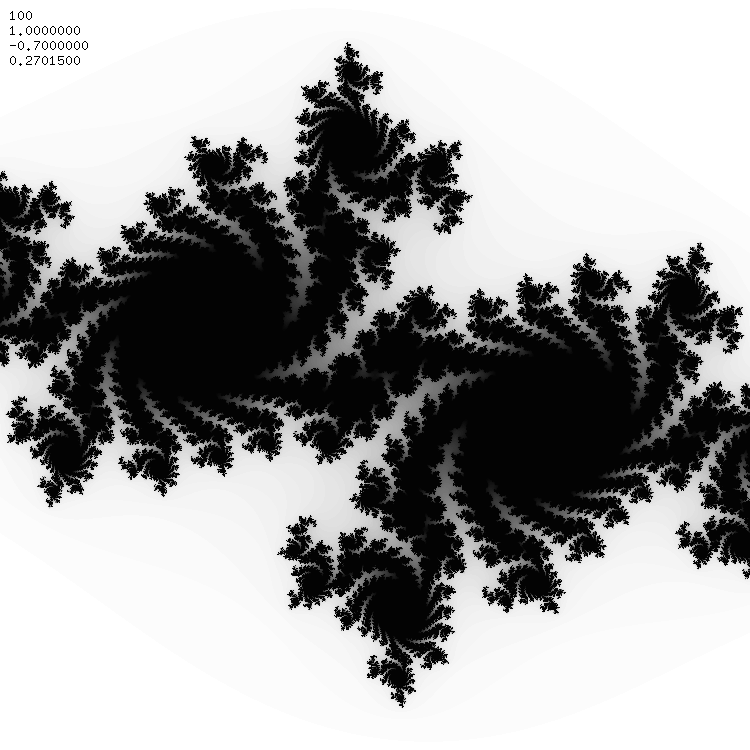
\includegraphics[width=0.75\linewidth]{images/Julia-Fractal.png}
		%for reference of this subfigure only
		\label{subfigure:Julia-Fractal}
	}
	\qquad
	\subfloat[Noise für Tinteneffekte]{
		
\includegraphics[width=0.75\linewidth]{images/Perlin-Coherent.png}
		%for reference of this subfigure only
		\label{subfigure:Perlin-Coherent}
	}
	\caption[
		Verschiedene Pixelgraphiken\newline
		% source url given in the table of figures
		\small\texttt{https://mediacube.at/wiki/}
	]{
		Verschiedene Pixelgraphiken
	}
	%for reference to all subfigures
	\label{figure:PixelImages}
\end{figure}

Unterstützte Pixelgraphikformate: PNG, JPEG, PDF.
Angabe von height oder width meist wichtig.

Referenz auf Abbildung \ref{figure:PixelImages} mit allen Teilbildern.
Referenz auf Unterabbildung \ref{subfigure:Julia-Fractal}.

%figure* stretches figure over both columns
\begin{figure*}[t]
	\centering
	
\includegraphics[width=0.9\textwidth]{images/KappaGamma.pdf}
	\caption{
		Vektorgraphik mit \LaTeX\ Beschriftung ($\kappa$, $\gamma$)
	}
	%for reference to this figure
	\label{figure:KappaGammaTau}
\end{figure*}

Referenz auf Abbildung \ref{figure:KappaGammaTau}.

Bei Vektorgraphik mit \LaTeX\ Beschriftung keine Skalierung mit width
oder height verwenden!
Vektorgraphik mit \LaTeX\ Beschriftung kann etwa mit \texttt{ipe} erstellt
werden.

Unterstütztes Vektorgraphikformat: PDF. EPS muss konvertiert werden.


\subsection{Unterabschnitt 2}
%for references to this subsection
\label{subsection:Coding}

\begin{lstlisting}[
	label=listing:Main, %for reference to this listing
	float=h,
	caption=main.cpp,
	firstnumber=10
]
int main(void) {
	while (true) {
	}
	return 0;
}
\end{lstlisting}

Wie man in Listing \ref{listing:Main} in Zeile 10 sieht, kann man die Zeilennummern im Listing absichtlich setzen, hier z.B. auf 10. In Listing \ref{listing:closure} wurde davon nicht Gebrauch gemacht. In diesem Fall beginnt die Nummerierung bei 1.

\begin{lstlisting}[
    label=listing:closure,
	float=h,
	caption=Closure in Javascript,
	language=JavaScript
]
function foo(x,y) {
    let i = x;
    return function(a) {
        return i * 2;
    }
}
\end{lstlisting}


\subsubsection{Unterunterabschnitt i}

Wörtliches Zitat:
%select proper language if not in German
\selectlanguage{english}
\begin{quote}
``Erwin Unruh discovered that templates can be used to compute
something at compile time. [...] The intriguing part of this exercise, however, was that the production of the prime numbers was performed by the compiler during the compilation process and not at run time.''

\autocite[305]{Bosch2014}
\end{quote}
%select German again or the language that you were using before (note ngerman stands for New German)
%\selectlanguage{ngerman}
\selectthesislanguage


\subsection{Unterabschnitt b}

\begin{enumerate}
	\item Punkt 1
	\begin{enumerate}
		\item Unterpunkt 1
		\item Unterpunkt 2
	\end{enumerate}
	\item Punkt 2
\end{enumerate}

\begin{itemize}
	\item Punkt 1
	\begin{itemize}
		\item Unterpunkt 1
		\item Unterpunkt 2
	\end{itemize}
	\item Punkt 2
\end{itemize}


\subsection{Unterabschnitt c}

\begin{table}[ht]
	\centering
	\begin{tabular}{r|rrr}
		    & $i$ & $j$ & $k$ \\ \hline
		$i$ &$-1$ & $k$ &$-j$ \\
		$j$ &$-k$ &$-1$ & $i$ \\
		$k$ & $j$ &$-i$ &$-1$
	\end{tabular}
	\caption{
		Multiplikationstabelle für Quaternionen
	}
	\label{table:Quaternions}
\end{table}

Referenz auf Tabelle \ref{table:Quaternions}.

\section{Abschnitt 2}
\label{section:MathematicalStuff}

Sei $f(x)$ eine stetige Funktion, so ist die \textbf{Fourier Transformierte}
$F(\omega)$ wie folgt definiert:
\begin{equation}
\label{equation:FourierDefinition}
	F(\omega) = \int_{-\infty}^{\infty} f(x) e^{-i\omega t} dt
\end{equation}

Referenz auf mathematische Gleichung (\ref{equation:FourierDefinition}).

Unnummerierte Gleichung:
\begin{equation*}
	e^{i\varphi} = \cos\varphi + i \sin\varphi
\end{equation*}
%you may also use \[ \] instead of \begin{equation*} and \end{equation*}

Gleichungssystem:
\begin{eqnarray}
	g(x) = f(x - x_0) & \Leftrightarrow &
		G(\omega) = F(\omega) e^{-i\omega x_0} \\
	g(x) = f(x) e^{i\omega_0 x} & \Leftrightarrow &
		G(\omega) = F(\omega - \omega_0)
\end{eqnarray}
